\documentclass[crop,tikz,convert={outext=.svg,command=\unexpanded{pdf2svg \infile\space\outfile}},multi=false]{standalone}

%math and margin packages
\usepackage{amsmath,amsfonts,amssymb,amsthm}
\DeclareMathOperator{\sech}{sech}
\usepackage{braket}
\usepackage[margin=1.0in]{geometry}
\usepackage{bbold}
\usepackage{braket}
\usepackage{ragged2e}
\usepackage{tikz}
\usetikzlibrary{angles,quotes}
\usepackage{tkz-euclide}
\usepackage[none]{hyphenat}
\usepackage{verbatim}
\usepackage{float}
\usepackage{wrapfig}
\usepackage{graphicx}
\usepackage{polynom}
\usepackage{longdivision}
\usepackage{bigints}
\usepackage{fontawesome}
\usepackage{pgfplots}
\usepackage{dirtytalk}
\allowdisplaybreaks


\begin{document}
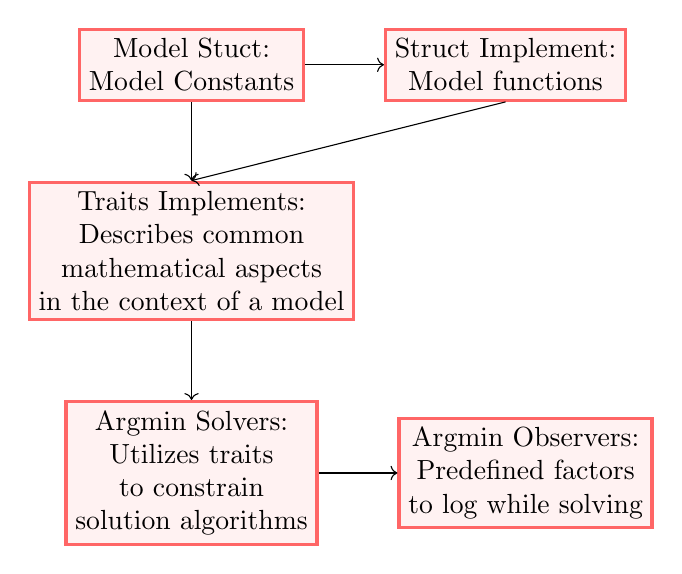
\begin{tikzpicture}[
	main/.style = {draw,circle},
	roundnode/.style={circle, draw=green!60, fill=green!5, very thick, minimum size=7mm},
	squarednode/.style={rectangle, draw=red!60, fill=red!5, very thick, minimum size=5mm},
]
\node[squarednode, align=center] (constants) {Model Stuct:\\ Model Constants};
\node[squarednode, align=center] (functions) [right=of constants]{Struct Implement:\\ Model functions};
\node[squarednode, align=center] (traits) [below=of constants]{Traits Implements:\\ Describes common\\ mathematical aspects\\ in the context of a model};
\node[squarednode, align=center] (solvers) [below=of traits]{Argmin Solvers:\\ Utilizes traits\\ to constrain\\ solution algorithms};
\node[squarednode, align=center] (observers) [right=of solvers]{Argmin Observers:\\ Predefined factors\\ to log while solving};

\draw[->](solvers.east)--(observers.west);
\draw[->](constants.east)--(functions.west);
\draw[->](constants.south)--(traits.north);
\draw[->](functions.south)--(traits.north);
\draw[->](traits.south)--(solvers.north);

\end{tikzpicture}\hspace{8mm}
\end{document}
